\begin{figure}
    \centering
    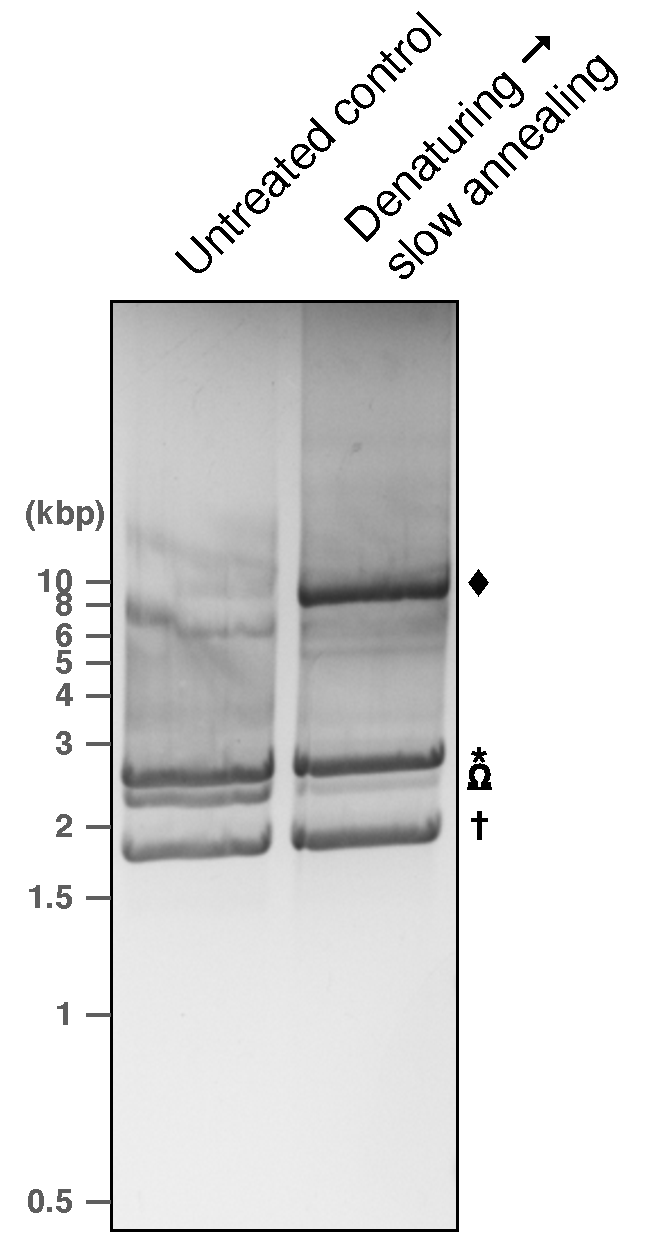
\includegraphics[width=0.4\textwidth]{chapters/figures/HybridGenotypingdsDNA.pdf}
    \caption{\textbf{Genotyping PCR products (using the genome of the heterozygous mNG-\gene{BubR1} HeLa-A12 cell line as the template) feature hybrid double-stranded DNAs that are thermodynamically unfavorable.}}
    Genotyping PCR products were purified using the GeneJET PCR Purification Kit and then equally split into 2 tubes. One of the tube (right lane) was then placed in boiling water bath for \SI{5}{min} and slowly cooled to room temperature, while the other tube (left lane) sit at room temperature over the entire period. The samples were then analyzed by 1\% agarose-TAE gel electrophoresis. Diamond: likely to be a certain higher-order origami complex. Asterisk: the PCR product of the edited mNG-\gene{BubR1} allele (\SI{2519}{bp}, confirmed by sequencing). Cross: the PCR product of the wildtype \gene{BubR1} allele (\SI{1793}{bp}, confirmed by sequencing). \underline{\textOmega{}} hybrid DNAs made up of one strand from the PCR product of the edited mNG-\gene{BubR1} allele and a complementary strand from the PCR product of the wildtype \gene{BubR1} allele. The identity of this band is also confirmed by sequencing (data not shown). Similar hybrid DNA likely also exist in the purified \gene{Mad1}-mNG genotyping PCR products \myref{GenotypingValidation}.
    \label{HybridGenotypingdsDNA}
\end{figure}







